% SECTION ====================================================================================
\vspace{-4pt}
\begin{sectionbox}
\section{Flüsse in Netzen}
% ============================================================================================
\subsection{Terminologie und Eigenschaften}\medskip
\textbf{Flussnetzwerk}\par
\begin{itemize}
    \item Flussnetzwerk $G=(V, E, c):$ gerichteter Graph mit Kapazitäten
    \item Antiparallele Kanten verboten
    \item Quelle $s$ und Senke $t:$ spezielle Knoten. Jeder Knoten $v$ liegt auf einem Pfad zwischen $s$ und $t: s \leadsto v \leadsto t$
\end{itemize}\par\smallskip
\begin{center}
    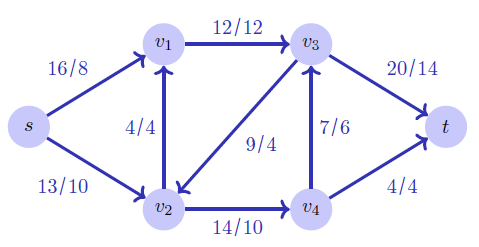
\includegraphics[width = 0.9\columnwidth]{../img/flussNet.png}
\end{center}

\textbf{Fluss}  $f: V \times V \rightarrow \mathbb{R}$ erfüllt Bedingungen:\par
\begin{itemize}
    \item \textbf{Kapazitätsbeschränkung}: $\forall u, v \in V: f(u, v) \leq c(u, v)$
    \item \textbf{Schiefsymmetrie}: $\forall u, v \in V: f(u, v)=-f(v, u)$
    \item \textbf{Flusserhaltung}: $u \in V \backslash\{s, t\}: \sum_{v \in V} f(u, v)=0$
    \item \textbf{Wert $w$ des Flusses}:$|f|=\sum_{v \in V} f(s, v)$
\end{itemize}\par\smallskip
\end{sectionbox}
\vspace{-4pt}
\begin{sectionbox}
\begin{cookbox}{Eigenschaften}
\item $|f|=f(s, V)$
\item $f(U, U)=0$
\item $f\left(U, U^{\prime}\right)=-f\left(U^{\prime}, U\right)$
\item $f(X \cup Y, Z)=f(X, Z)+f(Y, Z),$ wenn $X \cap Y=\emptyset$
\item $f(R, V)=0 \text { wenn } R \cap\{s, t\}=\emptyset . \text { [Flusserhaltung! }]$\smallskip
\par Wobei gilt:
\par $f\left(U, U^{\prime}\right):=\sum\limits_{u \in U \atop u^{\prime} \in U^{\prime}} f\left(u, u^{\prime}\right)$, $f\left(u, U^{\prime}\right):=f\left(\{u\}U^{\prime}\right)$
\end{cookbox}\medskip
\end{sectionbox}
\vspace{-4pt}
\begin{sectionbox}
\textbf{Restnetzwerk}\par
Restnetzwerk $G_{f}$ gegeben durch alle Kanten mit Restkapazität. Restnetzwerke haben dieselben Eigenschaften wie Flussnetzwerke, ausser dass antiparallele Kapazitäten-Kantenzugelassen sind.\par\smallskip
\begin{center}
    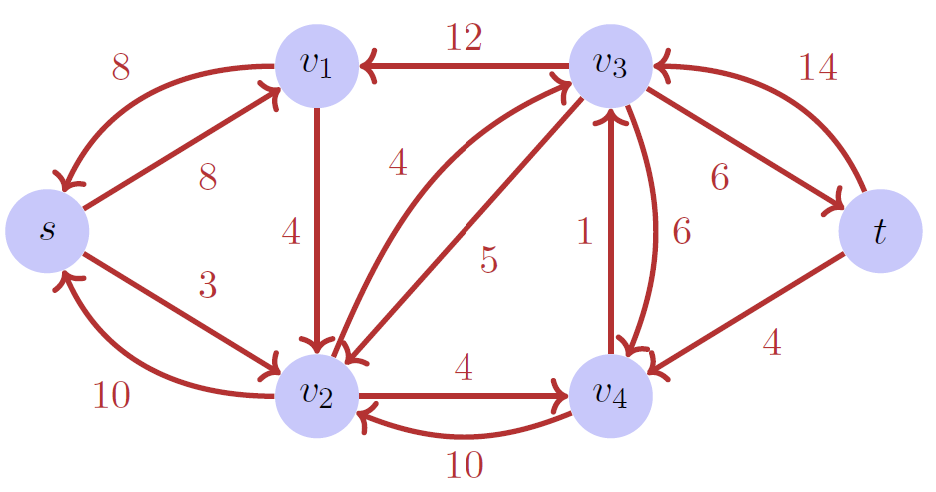
\includegraphics[width = 0.9\columnwidth]{../img/restNet.png}
\end{center}\par\smallskip

\textbf{Erweiterungspfade}\par
\begin{itemize}
    \item \textbf{Erweiterungspfad $p$}: einfacher Pfad von $s$ nach $t$ im Restnetzwerk $G_{f}$
    \item \textbf{Restkapazität} $c_{f}(p)=\min \left\{c_{f}(u, v):(u, v) \text { Kante in } p\right\}$
\end{itemize}

\end{sectionbox}
\vspace{-4pt}
\begin{sectionbox}
\subsection{Maximaler Fluss / Minimaler Schnitt}\smallskip
\begin{emphbox}
$|f| \leq \sum\limits_{v \in S, v^{\prime} \in T} c\left(v, v^{\prime}\right)=c(S, T)$
\end{emphbox}
Wobei $S$ die Menge der Knoten vor dem Cut und $T$ die Menge der Knoten nach dem Cut ist. Gezählt werden folglich nur die Kapazitäten von $S$ zu $T$ und nicht alle! So ergibt dies im Beispiel: $c(S,T)=12+7+4=23$\par\smallskip

\begin{center}
    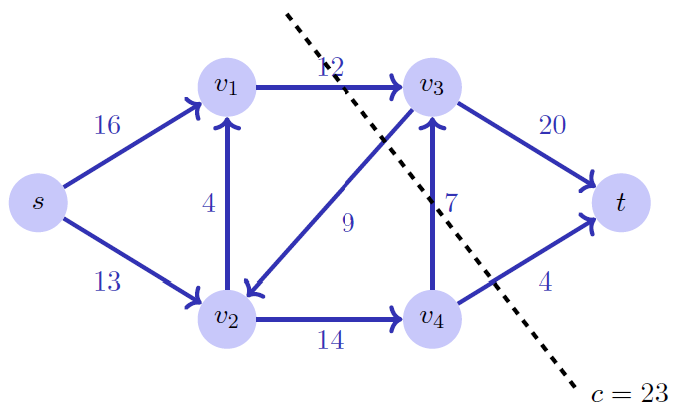
\includegraphics[width = 0.9\columnwidth]{../img/maxFlow.png}
\end{center}\par\smallskip

\begin{greenbox}
\textbf{Max-Flow Min-Cut Theorem}\par
Wenn $f$ ein Fluss in einem Flussnetzwerk $G=(V, E, c)$ mit Quelle $s$ und Senke $t$ ist, dann sind folgende Aussagen äquivalent:
\begin{enumerate}
    \item $f$ ist ein maximaler Fluss in $G$
    \item Das Restnetzwerk $G_{f}$ enthält keine Erweiterungspfade
    \item Es gilt $|f|=c(S, T)$ für einen Schnitt $(S, T)$ von $G$
\end{enumerate}
\end{greenbox}
\end{sectionbox}
\vspace{-4pt}
\begin{sectionbox}
\subsubsection{Die Ford-Fulkerson Methode}\smallskip
\begin{itemize}
    \item Starte mit $f(u, v)=0$ für alle $u, v \in V$
    \item Bestimme Restnetzwerk $G_{f}$ und Erweiterungspfad in $G_{f}$
    \item Erhöhe Fluss über den Erweiterungspfad
    \item Wiederholung bis kein Erweiterungspfad mehr vorhanden.
\end{itemize}\smallskip

\textbf{Ford-Fulkerson(G,s,t)}\par
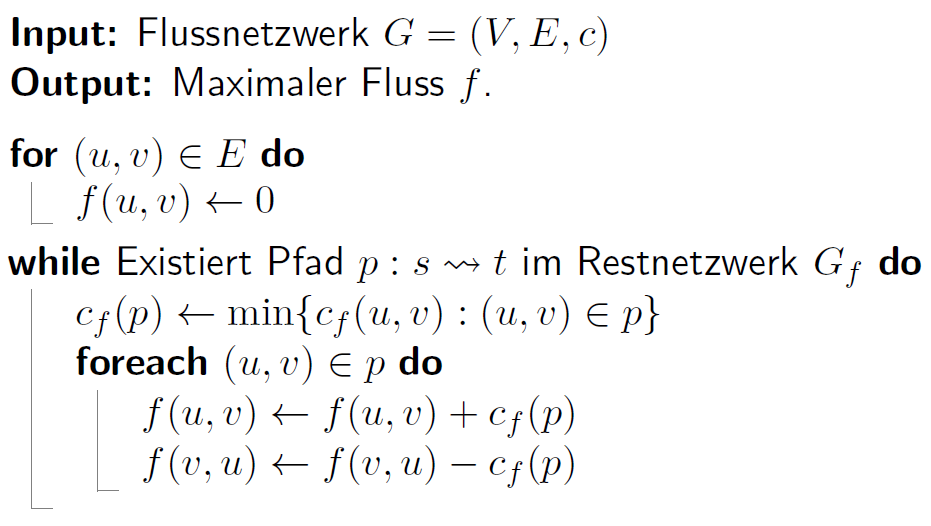
\includegraphics[width = 0.8\columnwidth]{../img/FoFu.png}\par\smallskip

\textit{Praktische Anmerkung zur Implementierung}\par
In einer Implementation des Ford-Fulkerson Algorithmus müssen die negativen Flusskanten nicht unbedingt gespeichert werden, da ihr Wert sich stets als der negierter Wert der Gegenkante ergibt. Somit kann dies vereinfacht folgendermassen implementiert werden:\par\smallskip
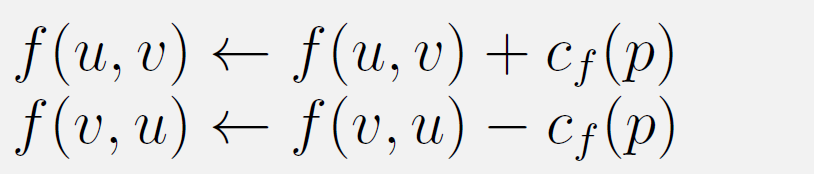
\includegraphics[width = 0.45\columnwidth]{../img/paFF1.png} wird zu
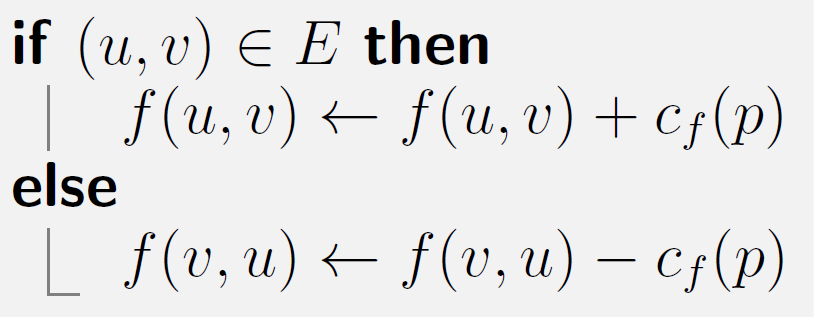
\includegraphics[width = 0.4\columnwidth]{../img/paFF2.png}\par\smallskip

\textbf{Analyse}\par
Der Ford-Fulkerson Algorithmus muss für irrationale Kapazitäten nicht einmal terminieren! Sonst $\mathcal{O}\left(f_{\max }\cdot |E|\right)$.
\end{sectionbox}
\vspace{-4pt}
\begin{sectionbox}
\subsubsection{Edmonds-Karp Algorithmus}\smallskip
Wähle in der Ford-Fulkerson-Methode zum Finden eines Pfades in $G_{f}$ jeweils einen Erweiterungspfad kürzester Länge (z.B. durch Breitensuche).\par $\Rightarrow$ Gesamte asymptotische Laufzeit: $\mathcal{O}\left(|V| \cdot|E|^{2}\right)$

\end{sectionbox}
\vspace{-4pt}
\begin{sectionbox}
\subsection{Bipartites Matching}\smallskip
Konstruiere zur einer Partition $L, R$ eines bipartiten Graphen ein korrespondierendes Flussnetzwerk mit Quelle $s$ und Senke $t,$ mit gerichteten Kanten von $s$ nach $L$, von $L$ nach $R$ und von $R$ nach $t$. Jede Kante bekommt Kapazität 1.\par
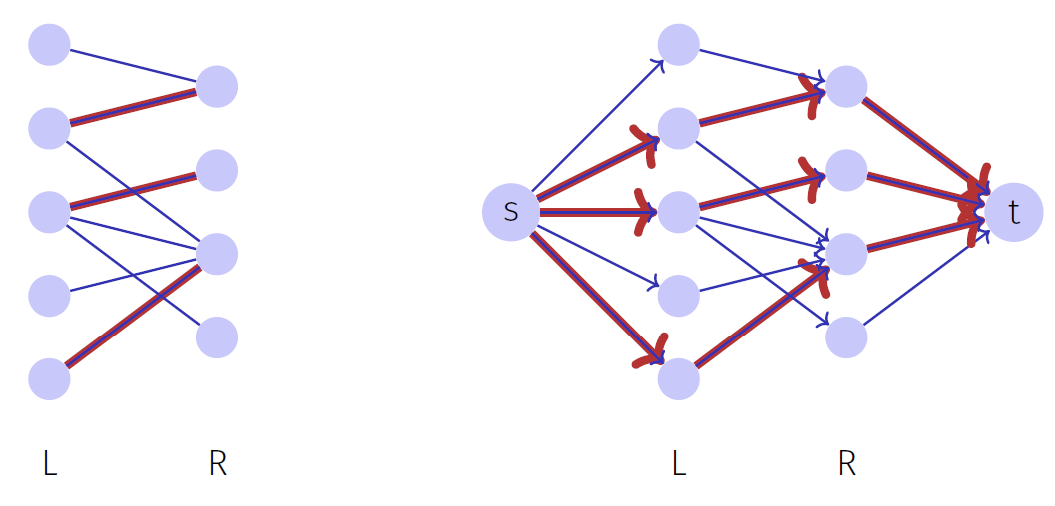
\includegraphics[width = \columnwidth]{../img/biMa.png}\par\smallskip
\end{sectionbox}
\vspace{-4pt}
\begin{sectionbox}
\subsection{Anwendungen vom Maximalen Fluss}\medskip

\textbf{Knotenkapazitäten in Graphen einbauen}\par
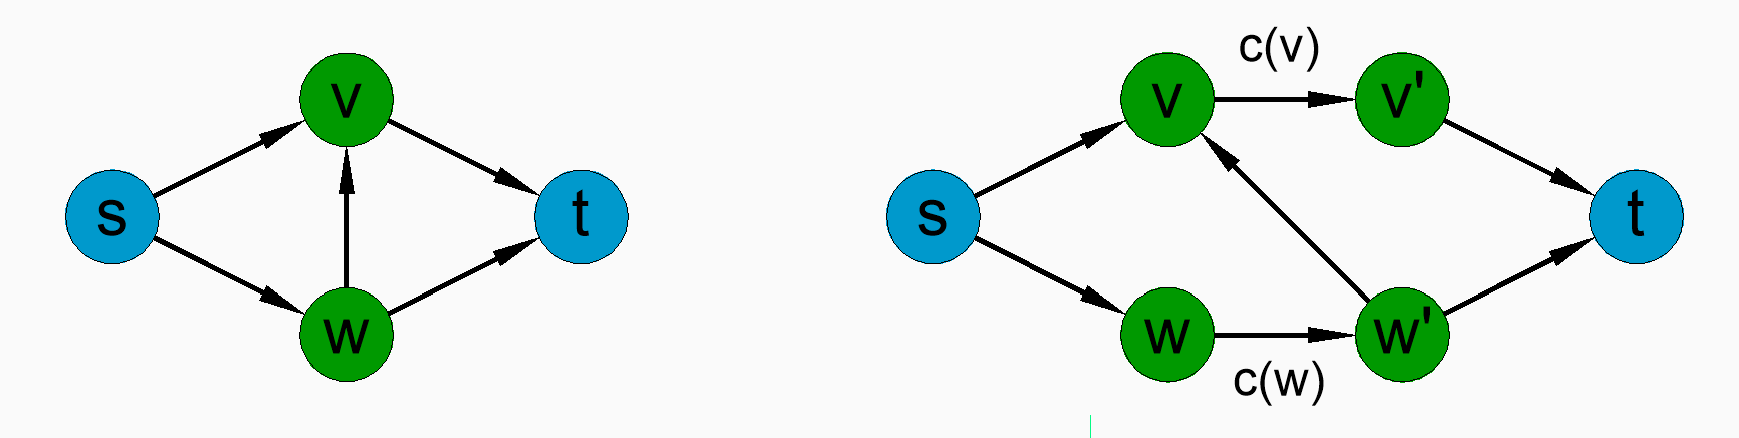
\includegraphics[width = \columnwidth]{../img/KontenKap.png}\par
\textit{Trick}: Um Knotenkapazitäten in einen Graphen einzubauen muss man aus einem Knoten zwei machen (\textbf{Input-Knoten} und \textbf{Output-Knoten}). Die Kante zwischen dem Input-Knoten und dem Output-Knoten muss die Kapazität des Knotens haben. D.h. $c(v) = c(v,v')$\par\smallskip
\end{sectionbox}